\section{Introduction}
%%
\subsection{Importance of the harmonic oscillator in physics}
The simplest example is a particle of mass $m$ moving in a potential which depends only on $x$ and has the form 
\begin{align*}
    V(x)=\frac{1}{2}kx^2,\quad k>0.
\end{align*}
\begin{figure}[h!]
    \centering
    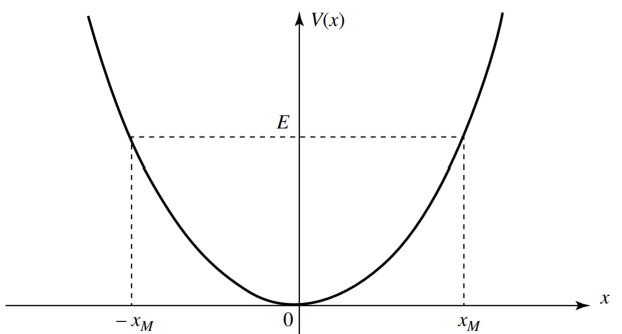
\includegraphics[width=.5\columnwidth]{PartOne/ChapterThree/potentialharmonicoscillator.png}
    \caption{Potential energy $V(x)$ of a 1D harmonic oscillator.}
\end{figure}
The particle is attracted towards the $x=0$ by a restoring force:
\begin{align*}
    F_x=\frac{dV}{dx}=-kx.
\end{align*}
In classical mechanics, the motion of the particle is a sinusoidal oscillation about $x=0$ with angular frequency $\omega=\sqrt{k/m}$.

\begin{emphasizer}[Various systems are governed by the harmonic oscillator equations]
    Whenever one studies the behavior of a system in the neighborhood of a stable equilibrium position, one arrives at equations which, 
    in the limit of small oscillations, are those of a harmonic oscillator.
\end{emphasizer}
%%
\subsection{The harmonic oscillator in classical mechanics}
The motion of the particle is governed by the dynamics equation
\begin{align}
    m\frac{d^2x}{dt^2}=-\frac{dV}{dx}=-kx\longrightarrow x=x_M\cos(\omega t-\varphi).
\end{align}
The kinetic energy of the particle is 
\begin{align}
    T=\frac{1}{2}m\left(\frac{dx}{dt}\right)^2=\frac{p^2}{2m},
\end{align}
where $p=mv$ is the momentum of the paticle. The total energy is 
\begin{align*}
    E=T+V=\frac{p^2}{2m}+\frac{1}{2}m\omega^2x^2=\frac{1}{2}m\omega^2x^2_M.
\end{align*}

\begin{itemize}[itemsep=0pt,topsep=0pt]
    \item The potential can be expanded in Taylor's series around $x_0$:
    \begin{align*}
        V(x)=\underbrace{V(x_0)}_{a}+V'(x_0)(x-x_0)+\underbrace{\frac{1}{2!}V^{(2)}(x_0)}_{b}(x-x_0)^2+\underbrace{\frac{1}{3!}V^{(3)}(x_0)}_{c}(x-x_0)^3+\cdots
    \end{align*}
    The force derived from the potential in the neighborhood of $x_0$ is 
    \begin{align}
        F_x=-\frac{dV}{dx}=-2b(x-x_0)-3c(x-x_0)^2+\cdots
    \end{align}
    The point $x=x_0$ is a stable equilibrium for the particle: $F_x(x_0)=0$. In adittion, if the amplitude of the motion of the particle 
    about $x_0$ is sufficiently small, we can keep with the linear term only and we have a harmonic oscillator since the dynamics equation can be approximated by 
    \begin{align*}
        m\frac{d^2x}{dt^2}\approx-2b(x-x_0).
    \end{align*}
    For higher energies $E$, the particle will be in period but not sinusoidal motion (as signal in Fourier series) between the limits $x_1$ and $x_2$. We then say that we are dealing with an \bfemph{anharmonic oscillator}.
    \begin{figure}[h!]
        \centering
        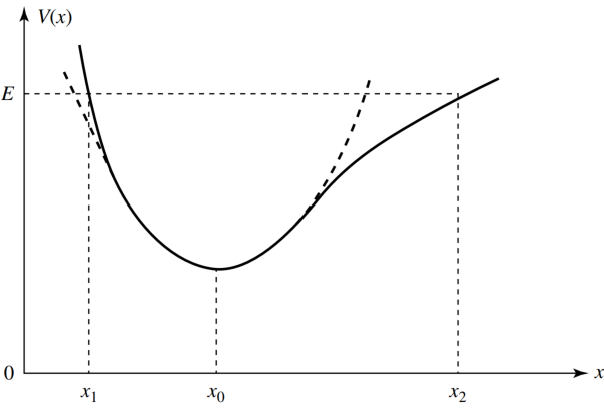
\includegraphics[width=.5\columnwidth]{PartOne/ChapterThree/taylorpotential.png}
        \caption{Any potential can be approximated by a parabolic potential. In $V(x)$, a classical particle of energy $E$ oscillates between $x_1$ and $x_2$.}
    \end{figure}
\end{itemize}
%
\subsection{General properties of the quantum mechanical Hamiltonian}
In QM, the classical quantities $x$ and $p$ are replaced respectively by the observables $X$ and $P$, which satisfy 
\begin{align*}
    [X,P]=i\hbar.
\end{align*}
It is then easy to obtain the Hamiltonian operator of the system from the total energy
\begin{align*}
    H=\frac{P^2}{2m}+\frac{1}{2}m\omega^2X^2.
\end{align*}
Since $H$ is time-independent (conservative system), the quantum mechanical study of the harmonic oscillator reduces to the solution of the eigenequation:
\begin{align*}
    H\ket{\varphi}=E\ket{\varphi}
\end{align*}
which is written, in the $\{\ket{x}\}$ representation 
\begin{align*}
    \left[-\frac{\hbar^2}{2m}\frac{d^2}{dx^2}+\frac{1}{2}m\omega^2x^2\right]\varphi(x)=E\varphi(x).
\end{align*}
Let us indicate some properties of the potential function:
\begin{itemize}[itemsep=0pt,topsep=0pt]
    \item\textbf{The eigenvalues of the Hamiltonian are positive}. If $V(x)$ has a lower bound, the eigenvalues $E$ of $H$ are greater than the minimum of $V(x)$:
    \begin{align*}
        V(x)\leq V_m\quad\text{requires}\quad E>V_m.
    \end{align*}
    We have chosen for the harmonic oscillator that $V_m=0$.
    \item\textbf{The eigenfunctions of $H$ have a definite parity} due to that $V(-x)=V(x)$ is an even function. We shall see that the eigenvalues of $H$ are not degenerate;
    the wave functions associated with the stationary tates are necessarily either even or odd.
    \item\textbf{The energy spectrum is discrete}. 
\end{itemize}